\documentclass[conference]{IEEEtran}
\usepackage{cite}
\usepackage{amsmath,amssymb}
\usepackage{booktabs}
\usepackage{multirow}
\usepackage{url}
\usepackage{graphicx}
\usepackage{pdfpages}

\title{Ensemble Learning for Customer Churn Prediction in Telecommunications}

\author{%
\IEEEauthorblockN{Ishmam Newaz, Author Two, Author Three, Author Four}
\IEEEauthorblockA{Rajshashi University of Engineering \&\& Technology\\
email: ishu.newaz@gmail.com\\
Author Two: affiliation@email.com; Author Three: affiliation@email.com; Author Four: affiliation@email.com}
}

\begin{document}
\maketitle

\begin{abstract}
Customer churn prediction is a core problem for subscription-based telecom services, where early identification of high-risk users can directly reduce revenue loss. This paper presents an ensemble-learning-based churn prediction pipeline built on the Telco Customer Churn dataset. We evaluate five ensemble strategies (soft voting, hard voting, stacking, bagging, and AdaBoost) under a leakage-controlled preprocessing setup. Experiments report hold-out test metrics, cross-validation performance, and repeated cross-validation confidence intervals. The best baseline ensemble is bagging with decision trees, which achieves test-set F1-score of 0.5825 and ROC-AUC of 0.8513. Threshold optimization improves bagging F1-score to 0.6427 and recall to 0.7166. Results indicate that threshold-aware ensemble deployment provides a practical performance gain for churn intervention systems.
\end{abstract}

\begin{IEEEkeywords}
Churn prediction, ensemble learning, telecom analytics, classification, threshold tuning
\end{IEEEkeywords}

\section{Introduction}
Customer churn prediction has significant operational value in the telecommunications industry. Because retention campaigns are costly, predictive models must balance precision and recall while maintaining stable generalization. Prior implementations in tabular churn datasets often overestimate performance due to target leakage. Therefore, robust feature filtering and cross-validation are required before model selection.

Ensemble learning is attractive in this context because it combines complementary model biases and often yields more stable performance than a single learner. Classical ensemble methods such as bagging and random forests reduce variance \cite{breiman1996bagging,breiman2001random}, while boosting methods focus on difficult samples \cite{freund1997adaboost,chen2016xgboost}. Stacking can further improve predictive quality by learning a meta-level combination of base models \cite{wolpert1992stacked}. However, in churn analytics, improvements in ranking quality (AUC) are not always equivalent to improvements in intervention quality (F1/recall at a selected threshold), which motivates a decision-focused evaluation strategy.

This study implements an end-to-end ensemble workflow and reports paper-ready metrics. Main contributions are:
\begin{enumerate}
\item A leakage-controlled preprocessing strategy for telecom churn data.
\item Comparative evaluation of multiple ensemble methods.
\item Cross-validation with confidence intervals for model stability.
\item Decision-threshold tuning to improve actionable churn recall.
\item A reproducible reporting pipeline with exported CSV results and figure assets.
\end{enumerate}

\section{Related Work}
Churn prediction has been studied across CRM and telecom domains for over a decade, with logistic regression and tree-based methods frequently used due to interpretability and tabular-data compatibility. Ensemble methods are now widely adopted when class imbalance and feature heterogeneity are present. Bagging-based approaches improve robustness under noisy predictors \cite{breiman1996bagging}, and boosting often improves ranking performance \cite{freund1997adaboost,chen2016xgboost}. In addition, stacking has been shown to improve generalization when base models capture different local decision boundaries \cite{wolpert1992stacked}.

Telecom-specific churn studies report that hybrid feature-selection and ensemble pipelines can substantially improve discrimination performance \cite{idris2013rotboost,keramati2014improved}. Interpretable and comprehensible churn modeling has also been emphasized for business adoption \cite{verbeke2011rule}. These findings motivate our choice of an ensemble-first workflow while preserving transparent reporting.

For model assessment, both ROC-AUC and precision-recall behavior are relevant in imbalanced classification. ROC analysis is threshold-independent \cite{fawcett2006roc}, while precision-recall analysis can better reflect positive-class retrieval quality under skewed distributions \cite{davis2006relationship}. Therefore, this paper reports both ranking-based metrics and thresholded metrics, then explicitly tunes the decision threshold for deployment realism.

From a methodological standpoint, ensemble learning foundations \cite{zhou2012ensemble} and imbalanced-learning literature \cite{he2009imbalanced,chawla2002smote} suggest that threshold selection and class-distribution-aware evaluation are as important as model architecture choices.

\section{Dataset and Preprocessing}
The experiment uses the \texttt{Telco\_customer\_churn.xlsx} dataset. The target variable is \texttt{Churn Value} (binary). Preprocessing includes:
\begin{itemize}
\item Numeric conversion of \texttt{Total Charges} with coercion and median imputation.
\item One-hot encoding for categorical attributes.
\item Removal of identifiers and leakage-prone fields (including raw and one-hot encoded churn-label/reason/score columns).
\item Stratified 80/20 train-test split with random state 42.
\end{itemize}

Leakage control is central in this dataset because several attributes can directly encode or proxy churn outcomes. During ablation, retaining churn-label-derived features yields unrealistically high scores. To avoid optimistic bias, both raw columns and one-hot-expanded leakage columns are removed prior to model training.

\section{Methodology}
\subsection{Base Learners}
Ensemble methods are built from logistic regression (with standardization), random forest, and XGBoost; additionally, tree-based bagging and AdaBoost are evaluated.

\subsection{Runtime and Reproducibility Settings}
The notebook supports two modes: a fast iteration mode and a full experimental mode. Fast mode uses lower estimator counts and fewer CV splits to reduce runtime and CPU load, while full mode increases estimator counts and repeated CV for publication-grade confidence estimates. Random seeds are fixed to 42 across splitters and estimators to ensure reproducibility.

\subsection{Ensemble Models}
The following models are implemented:
\begin{enumerate}
\item Soft Voting
\item Hard Voting
\item Stacking (meta-learner: logistic regression)
\item Bagging (decision tree base estimator)
\item AdaBoost
\end{enumerate}

\subsection{Evaluation Protocol}
Performance is measured using accuracy, precision, recall, F1-score, and ROC-AUC (when available). We report:
\begin{itemize}
\item Hold-out test set performance.
\item Stratified cross-validation means.
\item Repeated cross-validation confidence intervals.
\item Post-training threshold optimization for the best ensemble.
\end{itemize}

For binary churn classification, the key metrics are:
\begin{align}
\text{Precision} &= \frac{TP}{TP+FP}, \\
\text{Recall} &= \frac{TP}{TP+FN}, \\
F_1 &= 2 \cdot \frac{\text{Precision} \cdot \text{Recall}}{\text{Precision}+\text{Recall}}.
\end{align}
Because retention programs prioritize finding true churners, F1 and recall are treated as primary operational indicators.

\section{Results}
\subsection{Test Set Results}
\begin{table}[!t]
\centering
\caption{Test-set performance of ensemble models}
\label{tab:test_results}
\begin{tabular}{lccccc}
\toprule
Model & Accuracy & Precision & Recall & F1 & ROC-AUC \\
\midrule
Bagging (Tree) & 0.8006 & 0.6555 & 0.5241 & 0.5825 & 0.8513 \\
Stacking & 0.8041 & 0.6713 & 0.5134 & 0.5818 & 0.8502 \\
Voting (Hard) & 0.7991 & 0.6553 & 0.5134 & 0.5757 & -- \\
Voting (Soft) & 0.7842 & 0.6316 & 0.4492 & 0.5250 & 0.8293 \\
AdaBoost & 0.7346 & 0.0000 & 0.0000 & 0.0000 & 0.8268 \\
\bottomrule
\end{tabular}
\end{table}

Bagging and stacking provide the strongest F1-score among evaluated ensembles, with bagging slightly ahead.

\begin{figure}[!t]
\centering
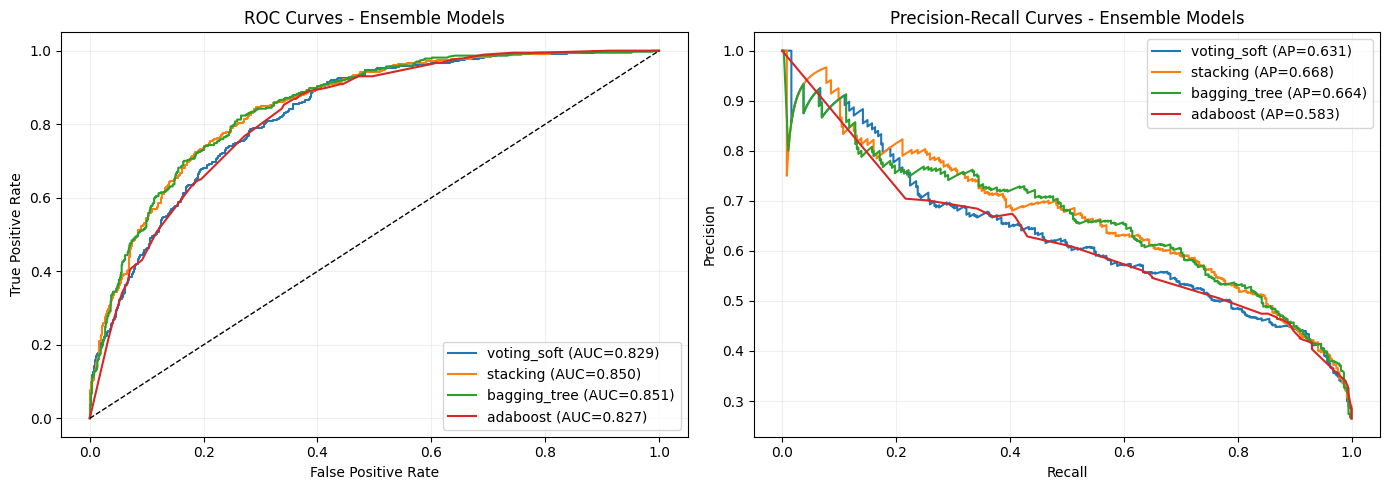
\includegraphics[width=\linewidth]{output.png}
\caption{ROC and Precision-Recall curves of evaluated ensemble models (exported from the experiment notebook).}
\label{fig:rocpr}
\end{figure}

Fig.~\ref{fig:rocpr} shows consistent ranking behavior with the tabled metrics. Curves indicate that bagging and stacking maintain stronger precision-recall behavior in the operating region relevant to churn intervention.

\subsection{Cross-Validation Stability}
\begin{table}[!t]
\centering
\caption{Cross-validation and repeated-CV confidence intervals}
\label{tab:cv_results}
\begin{tabular}{lccc}
\toprule
Model & CV F1 Mean & 95\% CI (F1) & CV ROC-AUC Mean \\
\midrule
Bagging (Tree) & 0.5829 & [0.5579, 0.6078] & 0.8546 \\
Stacking & 0.5818 & [0.5595, 0.6041] & 0.8529 \\
Voting (Hard) & 0.5600 & [0.5416, 0.5785] & -- \\
Voting (Soft) & 0.5332 & [0.5258, 0.5406] & 0.8282 \\
AdaBoost & 0.0000 & [0.0000, 0.0000] & 0.8371 \\
\bottomrule
\end{tabular}
\end{table}

Repeated-CV results confirm that bagging and stacking are both stable, with bagging showing a marginal advantage in F1.

The confidence-interval overlap between bagging and stacking indicates statistically similar performance under this feature set. Therefore, final selection should also consider training cost, serving latency, and threshold sensitivity.

\subsection{Threshold Optimization}
For the best ensemble (bagging), decision threshold optimization substantially improves recall and F1:
\begin{table}[!t]
\centering
\caption{Threshold tuning for bagging ensemble}
\label{tab:threshold}
\begin{tabular}{lcccc}
\toprule
Setting & Accuracy & Precision & Recall & F1 \\
\midrule
Default threshold (0.50) & 0.8006 & 0.6555 & 0.5241 & 0.5825 \\
Tuned threshold (0.38) & 0.7885 & 0.5826 & 0.7166 & 0.6427 \\
\bottomrule
\end{tabular}
\end{table}

Although accuracy decreases slightly, threshold tuning provides a meaningful F1 gain (+0.0602) and stronger recall, which is often preferred in churn prevention.

From a business perspective, this trade-off is often acceptable because false negatives (missed churners) are typically more costly than moderate increases in false positives.

\section{Discussion}
The experiments show three key observations:
\begin{enumerate}
\item Leakage control is essential; otherwise, unrealistically high scores can occur.
\item Ensemble methods outperform single-model baselines in stability and operational utility.
\item Threshold tuning is a low-cost, high-impact step for churn-focused decision systems.
\end{enumerate}

In practice, selecting a threshold depends on business cost trade-offs between false positives (unnecessary retention offers) and false negatives (missed churners).

\subsection{Threats to Validity}
Internal validity risks include residual feature leakage and split sensitivity. We mitigate these through explicit leakage-column filtering and stratified splitting. External validity may be limited because the study uses one telecom dataset and one static train-test partition. Construct validity is improved by reporting both threshold-independent metrics (ROC-AUC) and thresholded metrics (F1, recall, confusion matrix).

\subsection{Practical Deployment Notes}
For production deployment, probability calibration, drift monitoring, and periodic re-thresholding are recommended. A practical policy is to optimize threshold monthly against campaign budget constraints and observed churn prevalence.

\section{Conclusion}
This work presents a complete and reproducible ensemble-learning pipeline for telecom churn prediction. Under leakage-controlled preprocessing, bagging and stacking are the most competitive models. The best operational setup combines bagging with threshold tuning, achieving improved F1 and recall for retention-oriented deployment. Future work may include calibrated probabilities, cost-sensitive learning, and temporal validation on rolling churn windows.

\section*{Reproducibility Note}
All metrics in this paper are generated from the project outputs:\texttt{ensemble\_test\_scores.csv}, \texttt{ensemble\_cv\_scores.csv}, \texttt{ensemble\_repeated\_cv\_ci.csv}, and \texttt{ensemble\_threshold\_comparison.csv}.

\appendices
\section{Supplementary Graph Analysis}
The project workspace also contains a supplementary analysis PDF (\texttt{Graph analysis by cgpt.pdf}). For completeness, the first page is included below.

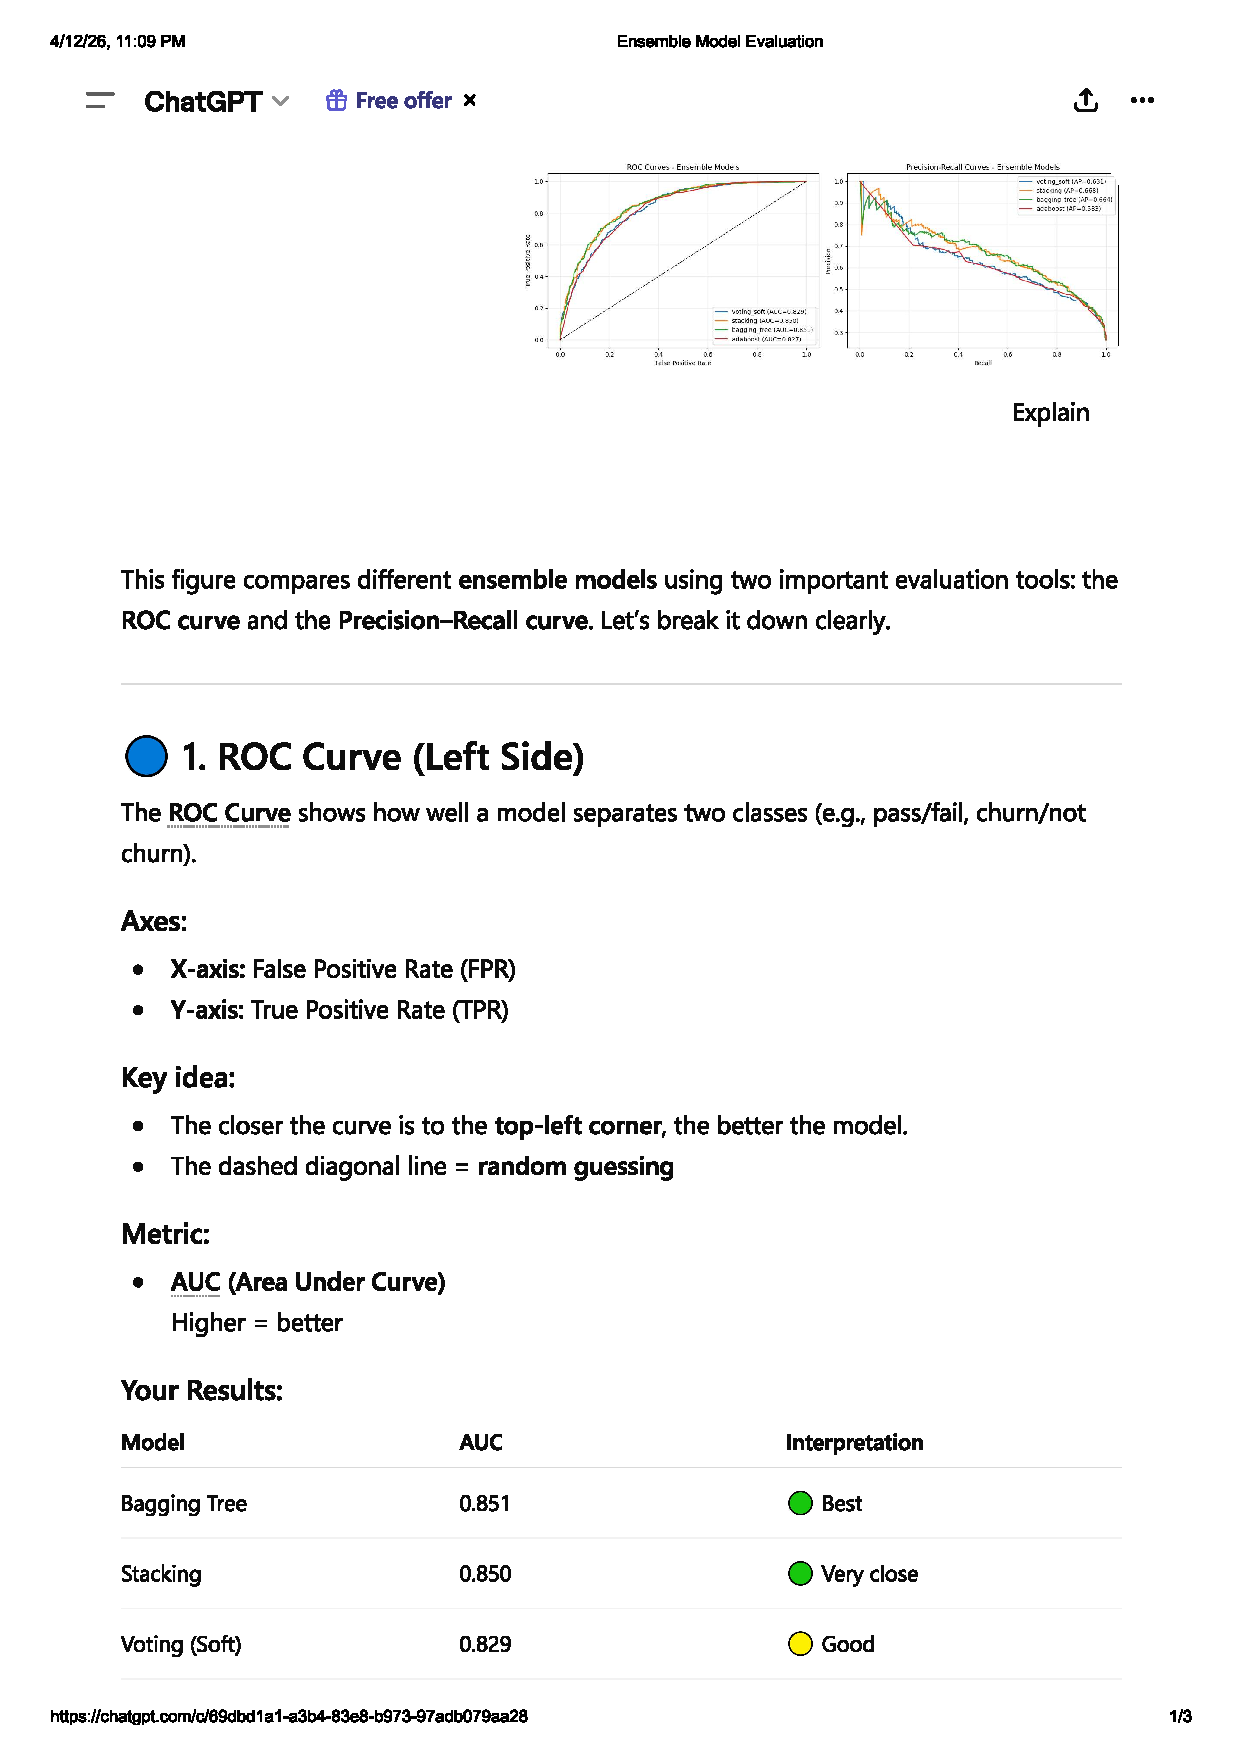
\includepdf[pages=1]{Graph analysis by cgpt.pdf}

\bibliographystyle{IEEEtran}
\bibliography{references}

\end{document}
